\documentclass[conference]{IEEEtran}
\IEEEoverridecommandlockouts
% The preceding line is only needed to identify funding in the first footnote. If that is unneeded, please comment it out.
\usepackage{cite}
\usepackage{amsmath,amssymb,amsfonts}
\usepackage{algorithmic}
\usepackage{graphicx}
\usepackage{textcomp}
\usepackage{xcolor}
\graphicspath{{../pdf/}{../jpeg/}{./figures/}}

\def\BibTeX{{\rm B\kern-.05em{\sc i\kern-.025em b}\kern-.08em
    T\kern-.1667em\lower.7ex\hbox{E}\kern-.125emX}}
\begin{document}

\title{Salt Detection Using Segmentation of Seismic Image
%{\footnotesize \textsuperscript{*}Note: Sub-titles are not captured in Xplore and
%should not be used}
%\thanks{Identify applicable funding agency here. If none, delete this.}
}

\author{\IEEEauthorblockN{%1\textsuperscript{st} 
		Mrinmoy Sarkar}
\IEEEauthorblockA{\textit{Department of Electrical \& Computer Engineering} \\
\textit{North Carolina A\&T State University}\\
Greensboro, NC-27411,  USA \\
msarkar@aggies.ncat.edu}
%\and
%\IEEEauthorblockN{2\textsuperscript{nd} Given Name Surname}
%\IEEEauthorblockA{\textit{dept. name of organization (of Aff.)} \\
%\textit{name of organization (of Aff.)}\\
%City, Country \\
%email address}
}

\maketitle

\begin{abstract}
In this project, we present state-of-the-art deep convolution neural network (DCNN) to segment seismic image for salt detection below the earth surface. Detection of salt location is very important for starting mining. Hence, seismic image is used to detect the exact salt location under the earth surface. However, precisely detecting the exact location of salt deposits is very difficult. Therefore, professional seismic imaging still requires expert human interpretation of salt bodies. This leads to very subjective, highly variable renderings. Hence, to create the most accurate seismic images and 3D renderings, we need a robust algorithm that automatically and accurately identifies if a surface target is salt or not. Since, the performance of DCNN is well-known and well-stablished for object recognition in image, DCNN is a very good choice for this particular problem. We successfully applied DCNN to a dataset of seismic images in which each pixel is labeled as salt or not. The result of this algorithm is promissing.
\end{abstract}

\begin{IEEEkeywords}
Seismic Image, Image Segmentation, DCNN, Auto-Encoder
\end{IEEEkeywords}

\section*{Objectives}
\begin{itemize}
	\item  Segmentation of seismic image into salt or sediment using DCNN.
	\item Automate the process of analysis of seismic image.
	\item Reduce the cost of identifying an earth surface before mining.
\end{itemize}

\section{Introduction}
A seismic image is produced from imaging the reflection coming from rock boundaries. The seismic image shows the boundaries between different rock types. In theory, the strength of reflection is directly proportional to the difference in the physical properties on either side of the interface. While seismic images show rock boundaries, they don't say much about the rock themselves; some rocks are easy to identify while some are difficult. There are several areas of the world where there are vast quantities of salt in the subsurface. One of the challenges of seismic imaging is to identify the part of subsurface which is salt. However, it is a image segmentation problem from the image processing perspective. There are many robust algorithms available for this task in the literature such as feature-space, image-domain and  physics based techniques \cite{lucchese2001colour}. These techniques have been successfully used for color image segmentation captured from digital camera. Since seismic images are significantly different than digital images, those state-of-the-art techniques fail for segmentation task. There are many challenges for seismic image segmentation. some of them are listed as follows:
\begin{itemize}
	\item Image capturing method.
	\item Uneven distribution of salt and other rocks.
	\item Rock which have density compared to salt.
	\item Only gray-level image means lack of information.
	\item Uneven structure of rocks below the earth surface which causes uneven reflection. 
\end{itemize}

However, there are many state-of-the-art machine learning technique that can be used to solve this problem. The most promissing technique in the literature is deep convolution neural network for any task related to image. This technique has been used for object recognition \cite{ren2015faster}, image segmentation \cite{chen2018deeplab}, style transformation \cite{etemad20093d}, human action recognition \cite{ji20133d}, medical image segmentation \cite{milletari2016v} and image denoising \cite{zhang2017beyond}. Hence, we have used this method to solve the problem at hand. In this work, our contributions are as follows:

\begin{itemize}
	\item We used state-of-the-art DCNN to segment seismic image for salt identification.
	\item We automated the post analysis of seismic images.
	\item We reduced the cost for seismic image analysis.
	\item We relaxed the necessity of human expert for seismic image segmantation.
\end{itemize}

The rest of the paper is organised as in section \ref{Literature survey} literature survey, in section \ref{Methodology} our method to solve the segmentation problem, in section \ref{Experimental Results} experimental results of our method and concludes with conclusion \& future work in section \ref{Conclusion Future Work}.

\begin{figure*}[!t]
	\centerline{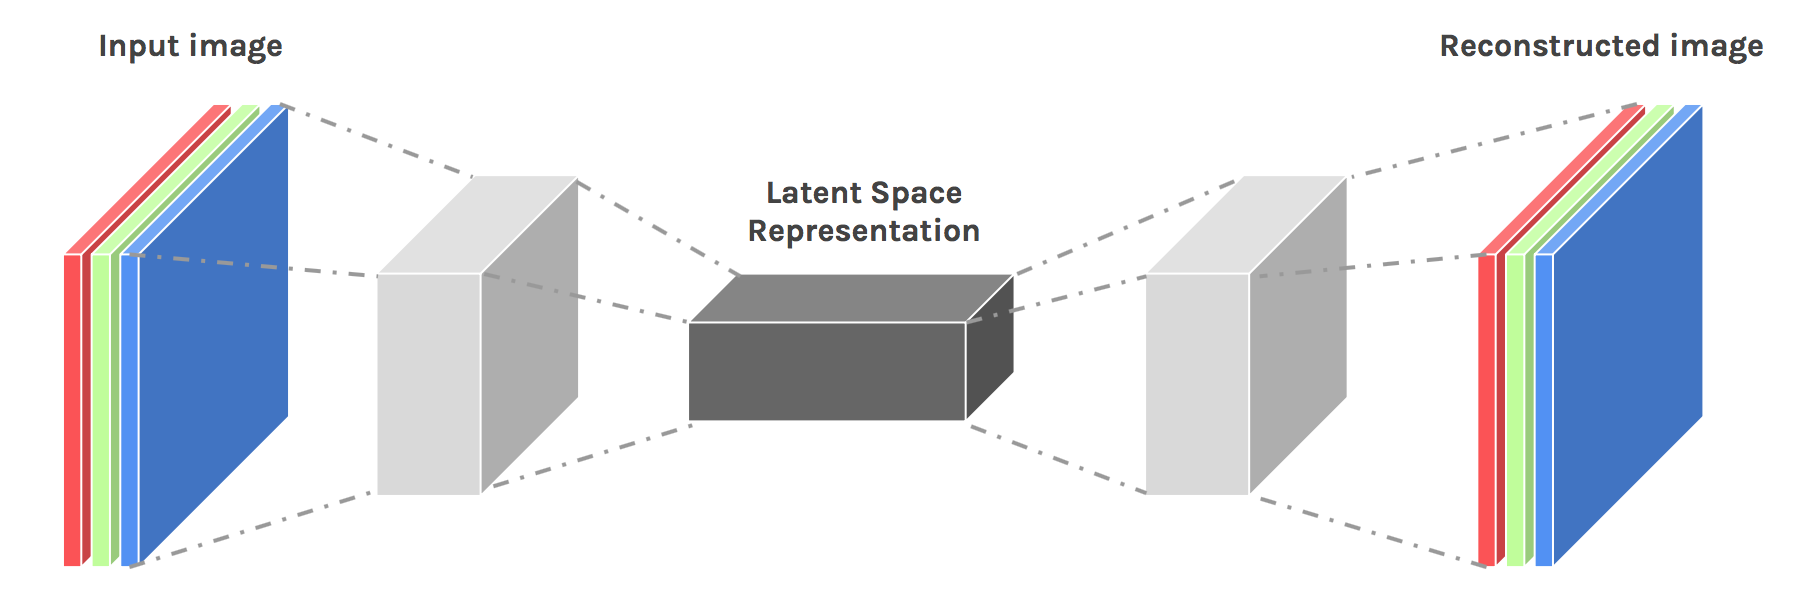
\includegraphics[width=7in, height=3.3in]{auto_encoder_architecture}}
	\caption{Convolutional Autoencoder architecture.\cite{autoencoder}}
	\label{fig:CAE}
\end{figure*}



\section{Literature survey}\label{Literature survey}
Image segmentation is a fundamental task for many image processing, video analysis or computer vision application. Hence, many research papers have been published on this topic. All the proposed method can be catagorised into the following three techniques \cite{lucchese2001colour}.
\begin{enumerate}
	\item Feature-Space Based Techniques
	\item Image-Domain Based Techniques
	\item Physics Based Techniques
\end{enumerate}

\subsection{Feature-Space Based Techniques} 
In this approach, color is assumed to be a constant property of the surface of each object within an image. So, every pixel can be clustered or grouped into some region within the image, which will produce the segmented image. Clustering and histogram thresholding are two well-known feature-space based techniques \cite{lucchese2001colour}.



\subsection{Image-Domain Based Techniques} 
The feature space based algorithms work on global property of the image which satisfy the homogenity requirement of image  segmentation. However, those techniques do not consider the spation characteristic of the image. Thue researchers found image domain based technique. These techniques satisfy both feature-space homogeneity and spatial compactness at the same time. The spatial compactness is ensured either by subdividing and merging or by progressively growing image regions, while the homogeneity is adopted as a criterion to direct these two processes. According to the strategy preferred for spatial grouping, these algorithms are usually divided into split-and-merge and region growing techniques.
Neural-network based classification, split and merge using region adjacency graph(RAG)  and edge based algorithmss are known to be image domain based techniques \cite{lucchese2001colour}.

\subsection{Physics Based Techniques} 
The discussed techniques are prone to segmentation error when the image is affected by highlights, shadowing and shadows. The problem can be solved considering the interaction of light with colored materials and to introduce models
of this physical interaction in the segmentation algorithms. This is the reason these techniques are known as physics based techniques. The mathematical tools used in these techniques are quite simillar to the previous two types of technique; the major difference with respect to those is the underlying physical model developed for the reflections properties of colored matter \cite{lucchese2001colour}.

As we are using seismic image, the images are not affected by shadowing or shawds. Our techniques lies in the image domain based techniques. However, the architechture and methodology is completely different than the techniques discussed in \cite{lucchese2001colour}. 



\section{Methodology}\label{Methodology}

In this project, we have used autoencoder(AE) architecture of neural network. Autoencoders (AE) are a family of neural networks for which the input is the same as the output. They work by compressing the input into a latent-space representation, and then reconstructing the output from this representation. If the architucture is built up on convolution neural networkthen it is known as Convolutional Autoencoder (CAE). Since out input is image, we used CAE to develop our segmentation model. The CAE architecture is shown in Fig. \ref{fig:CAE}. There are two parts of this architecture, named as encoder and decoder. The encoder part consist of convolution and pooling layers and the decoder part consists of convolution and upsampling layers. Each of these layers are describes in the following section.

\begin{figure}[!t]
	\centerline{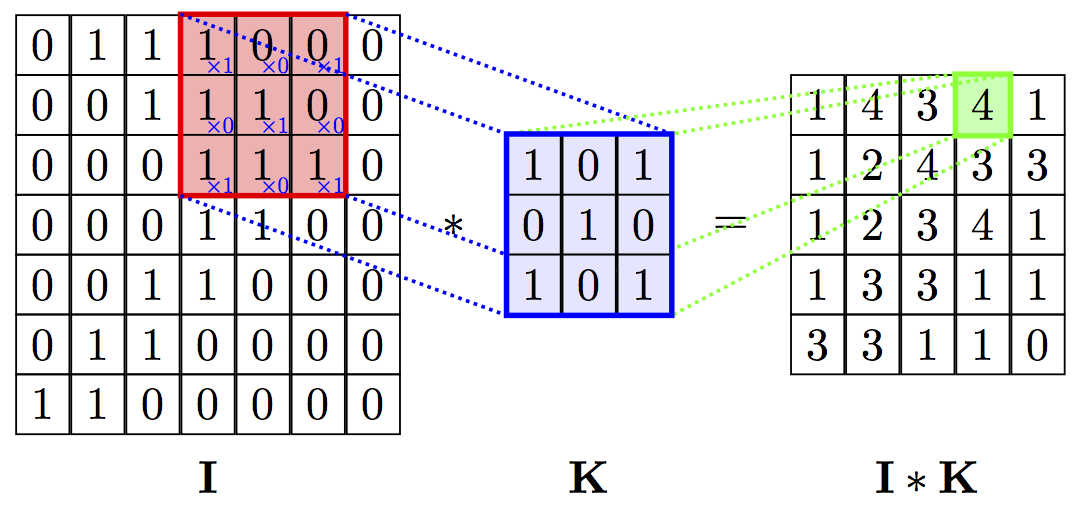
\includegraphics[width=3in, height=2in]{convlayer}}
	\caption{Convolution operation. \cite{conv2d}}
	\label{fig:conv_layer}
\end{figure} 

\begin{figure}[!t]
	\centerline{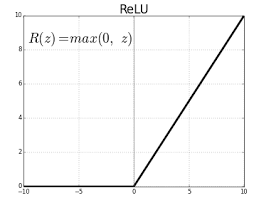
\includegraphics[width=3in, height=2in]{relu}}
	\caption{ReLU activation function. \cite{relu}}
	\label{fig:relu}
\end{figure} 

\subsection{Convolution Layer} 
The convolution layer is the main building block of CNN architecture. The primary purpose of convolution in case of a CNN is to extract features from the input image. Convolution preserves the spatial relationship between pixels by learning image features using small squares of input data. In this layer the input image is convolved with some predefined filters or kernel and then the output of the convolution operation is fed to an activation function. The $2D$ convolution operation is shown in Eqn. \ref{eqn:conv}. The output of the convolution operation is known as Feature Map. The size of the Feature Map is controlled by three parameters: \cite{anintuitivecnn}
\paragraph{Depth} Depth corresponds to the number of filters used for the convolution operation.
\paragraph{Stride} Stride is the number of pixels by which the filter matrix is slided over the input matrix. 
\paragraph{Zero-padding} Sometime zeros are padded around the border so that the filters can be applied to the bordering elements.

The convolution operation is shown in Fig. \ref{fig:conv_layer}. The last operation of a convolution layer is activation function. The most common activation function for CNN is rectified linear unit function (ReLU). The ReLU function is shown in Fig. \ref{fig:relu}.

\begin{equation}
f(m,n)\circledast g(m,n)=\sum_{j=-\infty}^{\infty}\sum_{i=-\infty}^{\infty}f(i,j)\times g(m-i,n-j)
\label{eqn:conv}
\end{equation}

\subsection{Pooling Layer}
A pooling layer is another building block of a CNN. Its function is to progressively reduce the spatial size of the representation to reduce the amount of parameters and computation in the network. Pooling layer operates on each feature map independently. The most common approach used in pooling is max pooling. The max pooling operation is shown in Fig. \ref{fig:pooling_layer}.

\subsection{Upsampling Layers}
In this layer the input image is resized to a higher dimention. There are different methods for resizing the image from lower dimention to higher dimention. One of those algorithms is nearest-neighbor algorithm. In this algorithm, the nearest pixels are copied from the original pixel value. For a scaling factor of 2 the output of nearest neighbor algorithm   is shown in Fig. \ref{fig:nearest_neighbor}.

\begin{figure}[!t]
	\centerline{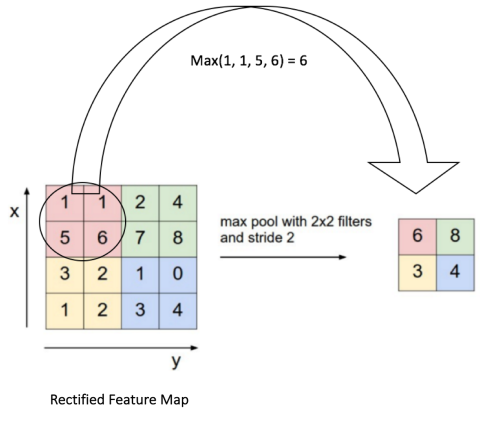
\includegraphics[width=2.5in, height=2.5in]{poolinglayer}}
	\caption{Operation in pooling layer. \cite{anintuitivecnn}}
	\label{fig:pooling_layer}
\end{figure}

\begin{figure}[!t]
	\centerline{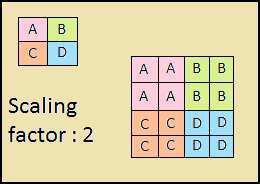
\includegraphics[width=2.5in, height=2.5in]{nearest_neighbor}}
	\caption{Image resizing (Nearest-Neighbor method). \cite{nearest_neighbour}}
	\label{fig:nearest_neighbor}
\end{figure}

\subsection{Architecture of the Developed Network}
The developed architecture is a combination of the three layers described above sections. The details of the architecture is given in Table \ref{tab:archi}.

\begin{table*}[!t]
	\centering
	\caption{Architecture of the developed Autoencoder model}
	\label{tab:archi}
	\begin{tabular}{llllllll}
		\hline
		&                  &                  &                  & Encoder          &                  &                &                  \\ \hline
		& layer1           & layer2           & layer3           & layer4           & layer5           & layer6         & layer7           \\ \hline
		Name                & conv2d           & max\_pooling2d   & conv2d           & max\_pooling2d   & conv2d           & max\_pooling2d & conv2d           \\ \hline
		No. of Filter       & 64               &                  & 64               &                  & 32               &                & 32               \\ \hline
		Filter dimension    & 3x3              &                  & 3x3              &                  & 3x3              &                & 3x3              \\ \hline
		Activation function & relu             &                  & relu             &                  & relu             &                & relu             \\ \hline
		Pool size           &                  & 2x2              &                  & 2x2              &                  & 2x2            &                  \\ \hline
		Stride size         &                  & 2x2              &                  & 2x2              &                  & 2x2            &                  \\ \hline
		& layer8           & layer9           & layer10          &                  &                  &                &                  \\ \hline
		Name                & max\_pooling2d   & conv2d           & max\_pooling2d   &                  &                  &                &                  \\ \hline
		No. of Filter       &                  & 16               &                  &                  &                  &                &                  \\ \hline
		Filter dimension    &                  & 3x3              &                  &                  &                  &                &                  \\ \hline
		Activation function &                  & relu             &                  &                  &                  &                &                  \\ \hline
		Pool size           & 2x2              &                  & 2x2              &                  &                  &                &                  \\ \hline
		Stride size         & 2x2              &                  & 2x2              &                  &                  &                &                  \\ \hline
		&                  &                  &                  & Decoder          &                  &                &                  \\ \hline
		& layer11          & layer12          & layer13          & layer14          & layer15          & layer16        & layer17          \\ \hline
		Name                & upsampler        & conv2d           & upsampler        & conv2d           & upsampler        & conv2d         & upsampler        \\ \hline
		No. of Filter       &                  & 16               &                  & 32               &                  & 32             &                  \\ \hline
		Filter dimension    &                  & 3x3              &                  & 3x3              &                  & 3x3            &                  \\ \hline
		Activation function &                  & relu             &                  & relu             &                  & relu           &                  \\ \hline
		Output Image size   & 8x8              &                  & 16x16            &                  & 32x32            &                & 64x64            \\ \hline
		Resize method       & Nearest Neighbor &                  & Nearest Neighbor &                  & Nearest Neighbor &                & Nearest Neighbor \\ \hline
		& layer18          & layer19          & layer20          & layer21          & layer22          & layer23        &                  \\ \hline
		Name                & conv2d           & upsampler        & conv2d           & downsampler      & conv2d           & output         &                  \\ \hline
		No. of Filter       & 64               &                  & 64               &                  & 1                &                &                  \\ \hline
		Filter dimension    & 3x3              &                  & 3x3              &                  & 3x3              &                &                  \\ \hline
		Activation function & relu             &                  & relu             &                  &                  & sigmoid        &                  \\ \hline
		Output Image size   &                  & 128x128          &                  & 101x101          &                  &                &                  \\ \hline
		Resize method       &                  & Nearest Neighbor &                  & Nearest Neighbor &                  &                &                  \\ \hline
	\end{tabular}
\end{table*}



\subsection{Loss function}
To train the network, reduce mean of sigmoid cross entropy is used as the loss function. If $x$ is the predicted label and $z$ is the true label then the sigmoid cross entropy can be written as equation \ref{eqn:sigmoid_cross_entropy} and if $z$ is a set of $n$ different values and $m$ is the total  number of training samples then the reduce mean loss can be calculated using equation \ref{eqn:loss}.

\begin{equation}
\begin{split}
&sigmoid\_cross\_entropy(x,z) \\
&= z\times (-\log(sigmoid(x)) )\\
 &+ (1-z)*(-\log(1-sigmoid(x)))
\end{split}
\label{eqn:sigmoid_cross_entropy}
\end{equation}  


\begin{equation}
sigmoid(x) =\frac{1}{1+e^{-x}}
\label{eqn:sigmoid}
\end{equation}  


\begin{equation}
\begin{split}
&Loss = \frac{1}{m}\times\sum_{j=1}^{m}\sum_{i=1}^{n}sigmoid\_cross\_entropy_j(x_i,z_i) 
\end{split}
\label{eqn:loss}
\end{equation} 

\subsection{Training Algorithm}
The training algorithm used for optimizing the pre-defined loss function is ADADELTA. As describes in \cite{zeiler2012adadelta}, the ADADELTA is an adaptive gradient descent algorithm which adapts the learning rate dynamically during the training process based on first order information only and the computational cost of the algorithm is less than any other state-of-the-art gradient descent algorithm. For more information about this optimization technique, readers can look into \cite{zeiler2012adadelta}.

\begin{figure}[!t]
	\centerline{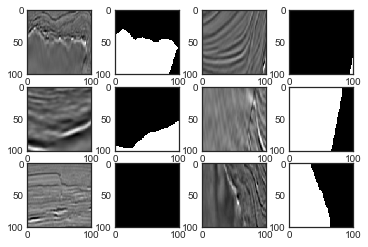
\includegraphics[width=3.5in, height=2.5in]{dataset}}
	\caption{Sample seismic images and corresponding mask images. }
	\label{fig:dataset}
\end{figure}
\section{Experimental Results}\label{Experimental Results}
The dataset used for this project, contains 4000 seismic images with 4000 labeled mask images. The seismic images are in gray scale and the mask images are in black and white. White pixel in mask image indicated the presence of salt in original image. The size of all the images are $101\times101$. The input images are resized to $128\times128$ for the sake of fast computation but the mask images are keep unchanged. Some sample seismic and mask images are shown in Fig. \ref{fig:dataset}. The data set is obtained from \cite{tsg}. Software tools used for this project, are listed below:

\begin{enumerate}
	\item Python
	\item scikit-learn
	\item TensorFlow
	\item Keras
	\item Pandas
	\item Numpy
	\item Matplotlib
\end{enumerate}

With an initial learning rate of 0.001 and with a mini batch size of 100, after 5000 epoches the training loss was 0.3297 and the test loss was 0.3464. However, after 10000 epoches the training loss was 0.2406 and the test loss is 0.2666.



\section{Conclusion \& Future Work}\label{Conclusion Future Work}











%\begin{table}[htbp]
%\caption{Table Type Styles}
%\begin{center}
%\begin{tabular}{|c|c|c|c|}
%\hline
%\textbf{Table}&\multicolumn{3}{|c|}{\textbf{Table Column Head}} \\
%\cline{2-4} 
%\textbf{Head} & \textbf{\textit{Table column subhead}}& \textbf{\textit{Subhead}}& \textbf{\textit{Subhead}} \\
%\hline
%copy& More table copy$^{\mathrm{a}}$& &  \\
%\hline
%\multicolumn{4}{l}{$^{\mathrm{a}}$Sample of a Table footnote.}
%\end{tabular}
%\label{tab1}
%\end{center}
%\end{table}

%\begin{figure}[htbp]
%\centerline{\includegraphics{fig1.png}}
%\caption{Example of a figure caption.}
%\label{fig}
%\end{figure}



%\section*{Acknowledgment}

%\section*{References}



\bibliographystyle{IEEEtran}
\bibliography{refs}

\end{document}
